\documentclass[onecolumn,conference]{IEEEtran}
 \usepackage{enumitem}
\usepackage[document]{ragged2e}
\usepackage{blindtext}
\usepackage{graphicx}

\title{Joint Radar Communication System using OFDM}

\author{

\IEEEauthorblockN{Owen Sowatzke}
\IEEEauthorblockA{\textit{Electrical Engineering Department} \\
\textit{University of Arizona}\\
Tucson, USA \\
osowatzke@arizona.edu}

\and
\IEEEauthorblockN{Iman Miraki}
\IEEEauthorblockA{\textit{Electrical Engineering Department} \\
\textit{University of Arizona}\\
Tucson, USA \\
imanmiraki@arizona.edu}}

\begin{document}
	\maketitle
\setlength{\hsize}{0.9\hsize}% emphasize effects
\RaggedRight
\section {Introduction}
     Vehicle-to-Vehicle networks seek to enhance road safety and reduce traffic congestion by sharing information between vehicles. Such networks possess enormous potential in improving driving safety and traffic conditions by sharing road and traffic information among vehicles in real-time.These systems need dedicated bandwidth to avoid delays associated with third party networks. Sharing bandwidth between existing vehicle radar and planned communication network would reduce total bandwidth usage and power consumption.\par
     The Idea behind JRC is to integrate radar sensing and wireless communication systems into a single framework, allowing vehicles to perform both tasks using the same hardware, spectrum, and waveform resources. This integration is critical for improving situational awareness, safety, and efficient use of spectrum in V2V networks.\par
     In this paper, we design a joint-radar communication (JRC) system, which uses OFDM for communication and zero-forcing to generate a range response from the OFDM returns. To evaluate the system performance, we provide the simulation results and compare Radar and Communication with JRC.

	\begin{enumerate}
		\item Radar
          \item OFDM
        \item JRC\par
        
   \section {Radar}

     \section {OFDM}
Random bits are generated and modulated using QPSK. These symbols are mapped onto sub-carriers, excluding pilots and zero carriers.
Pilots are inserted at regular intervals and zero carriers are placed at the edges of the spectrum.The IFFT converts the frequency domain symbols to the time domain. A Hamming window is applied to each OFDM symbol to reduce spectral leakage. Acyclic prefix is added to teh windowed OFDM symbols to mitigate ISI. The AWGN channel is used to transmit the flattened signal to the receiver.\par
The receiver removes the cyclic prefix. The data subcarriers are extracted and demodulated from FFT results in frequency domain. The received bits are compared to the transmitted bits to calculate the BER fo reach SNR value. 
\begin{figure}
    \centering
    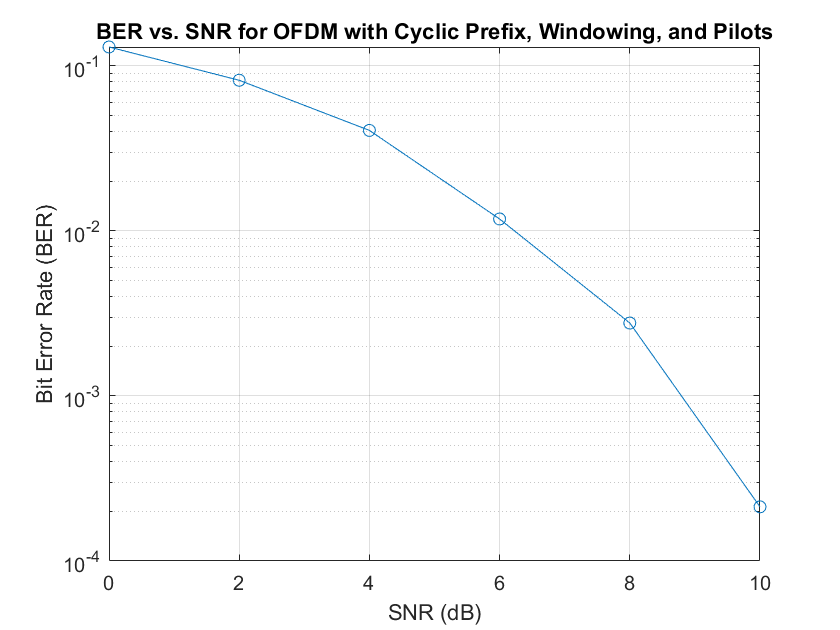
\includegraphics[width=0.5\linewidth]{OFDM_BER.jpg}
    \caption{OFDM BER vs SNR}
    \end{figure}
\begin{figure}
        \centering
        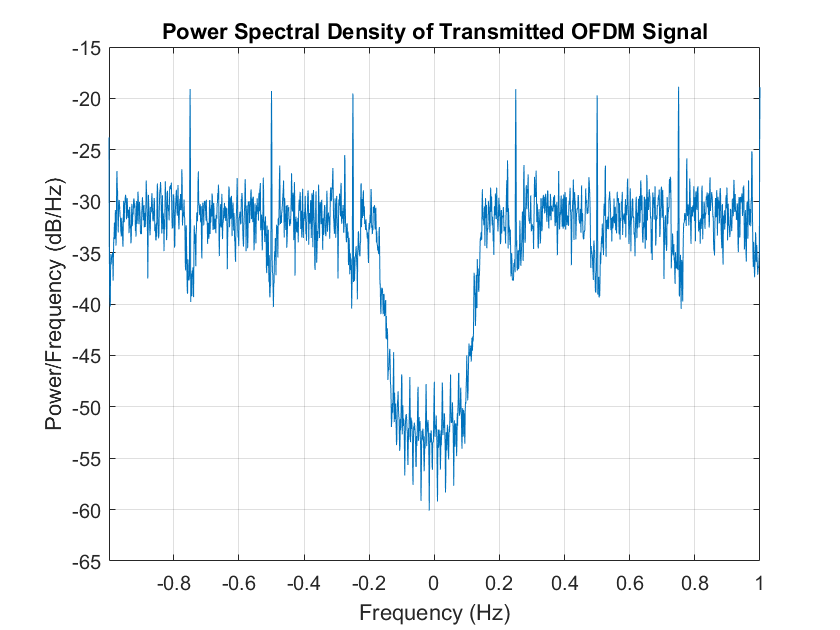
\includegraphics[width=0.5\linewidth]{OFDM_PowerSpectralDensity.jpg}
        \caption{OFDM Power Spectral Density}
    \end{figure}
        

  


     \section {JRC}

	\end{enumerate}
	
	\nocite{yang_subcarrier_multiplexing}
	\bibliography{sources}{}
    \bibliographystyle{ieeetr}
  
\end{document}
